\documentclass[10pt,a4paper]{article}
\usepackage[utf8]{inputenc}
\usepackage{amsmath}
\usepackage{amsfonts}
\usepackage{amssymb}
\usepackage{palatino}
\usepackage[left=2.5cm,right=2.5cm,top=2.5cm,bottom=2.5cm]{geometry}
\usepackage{geometry}
\usepackage{listings}
\usepackage{amsmath,amsthm}
\usepackage{extpfeil}
\usepackage{indentfirst}
\usepackage{mathptmx}
\usepackage{subfig}
\usepackage{graphicx}
\usepackage{hyperref}
\usepackage{diagbox}
\usepackage{cite}
\global\long\def\d{\text{d}}
\newtheorem{proposition}{Proposition}
\newtheorem{definition}{Definition}
\newtheorem{corollary}{Corollary}
\newtheorem{claim}{Claim}
\newtheorem{theorem}{Theorem}
\newtheorem{lemma}{Lemma}
\newtheorem{fact}{Fact}
%\usepackage{booktabs}
%\usepackage{lipsum}
\title{DSGA-1011 Natural Language Processing with Representation Learning Homework 2
}
\author{Xintian Han (xh1007)}
\begin{document}
\maketitle
\section{SNLI Classification} 
We build CNN and RNN encoders together with a fully-connected network to solve the 3-class classification problem in SNLI. We use an encoder (either a CNN or an RNN) to map each string of text (hypothesis and premise) to a fixed-dimension vector representation. We concatenate or multiply the two representations and feed them through a network of 2 fully-connected layers with a ReLU activation. We use pretrained word embeddings from fast-Text to embed our word tokens. We retrain the embedding of UNK token in our task. For the CNN, we use a 2-layer 1-D convolutional network with ReLU activations. For the RNN, we use a single-layer, bi-directional GRU and take the last hidden state as the encoder output. (We sum up the hidden states from two directions.) The embedding size is 300 when we use pretrained fast-Text word vectors. We use the following set of hyperparameters for RNN and CNN.
\begin{itemize}
\item The size of the hidden dimension of the CNN and RNN \texttt{hidden\_size}: 300, 400, 500.
\item The kernel size of the CNN \texttt{kernel\_size}: 3,5 (For kernel size 3, we use padding = 3 and for kernel size 5, we use padding = 5.)
\item Different ways of interacting the two encoded sentences \texttt{is\_concat}: concatenation and element-wise multiplication.
\item Regularization: weight decay \texttt{is\_wd} and dropout \texttt{is\_dropout}.
\end{itemize}
Some fixed hyperparameters are optimizer (ADAM), learning rate (initial learning rate = 0.0001 and the $i$-th epoch has the learning rate initial learning rate/ $i$), fixed hidden dimension \texttt{hid\_dim}= 300 in fully-connected network. We use max sentence length 50 which is greater than 95\% quantile of the whole sentence lengths. All networks we trained for 10 epochs.
\subsection{Vary Hidden Sizes}
We first use dropout, no weight decay, element-wise multiplication and kernel size 3. We vary hidden size for both RNN and CNN. We also choose the best model that has the best validation accuracies during each epoch of training. The results are in Table \ref{tab: hid} and Figure \ref{fig: hid}. The title of the figure for train and validation loss and accuracy curves are: \\
\noindent`loss\_' and `acc\_' plus `\texttt{encoder\_hidden\_size\_hid\_dim\_is\_concat\_kernel\_size\_is\_wd\_is\_dropout}'. \\
 We find that hidden size 300 is the best for CNN and 400 for RNN. Actually, hidden size 300 and 400 for CNN have the same validation accuracy, but due to the Occam's razor, we choose the one with lower hidden size. Higher hidden size will have higher train accuracy but may have poorer generalization. Here the lowest hidden size is the best for CNN. For RNN, we notice that when hidden size = 500, the training may not converge. But due to the limit time and resources, we train each model 10 epochs. So our best choice for hidden size of RNN is 400. It is faster than 500 but more accurate than 300 when training 10 epochs.
\begin{table}[!ht]
\centering
\begin{tabular}{|c|c|c|c|c|c|c|}
\hline
Network & \multicolumn{3}{|c|}{CNN} & \multicolumn{3}{|c|}{RNN} \\ \hline
hidden size& 300 & 400 & 500& 300 & 400 & 500\\\hline
validation accuracy& \textbf{62.3} & 62.3 & 62.1 & 73.6 & \textbf{73.9} & 64.2\\ \hline
number of parameters & 632103 & 962303 & 1352503 & 1175103 & 1806303 & 2557503 \\ \hline 
\end{tabular}
\caption{\label{tab: hid}Accuracy on Validation Set and Number of Parameters When We Vary Hidden Sizes, and Fix the Others.}
\end{table}
\begin{figure}[!ht]
\centering
\subfloat[300 CNN]{
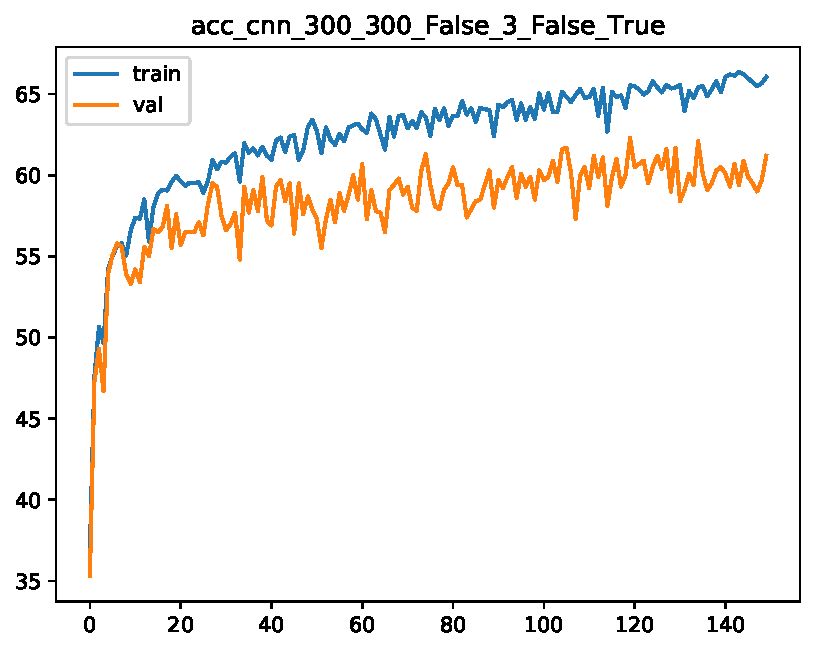
\includegraphics[width = 2.5cm]{acc_cnn_300_300_False_3_False_True.pdf}
}
\subfloat[400 CNN]{
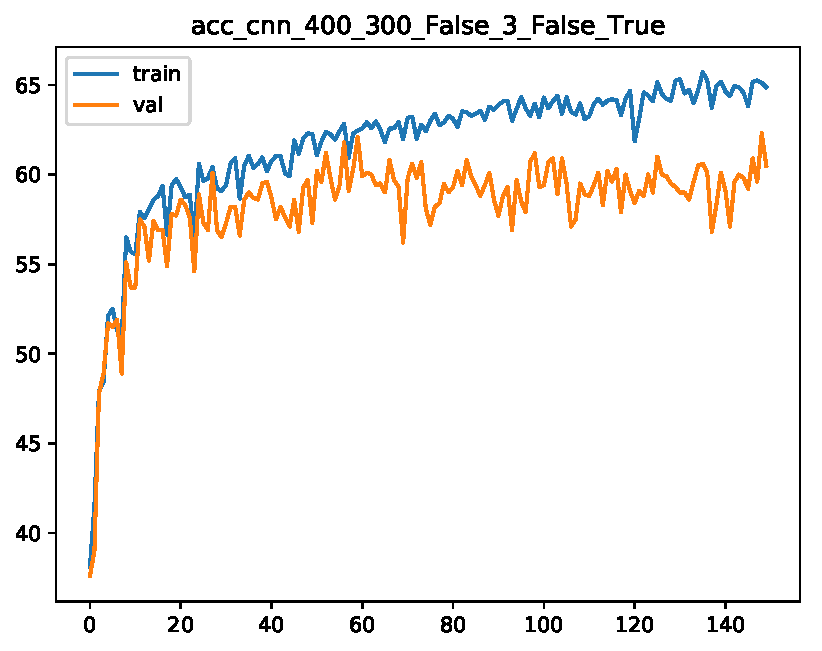
\includegraphics[width = 2.5cm]{acc_cnn_400_300_False_3_False_True.pdf}
}	
\subfloat[500 CNN]{
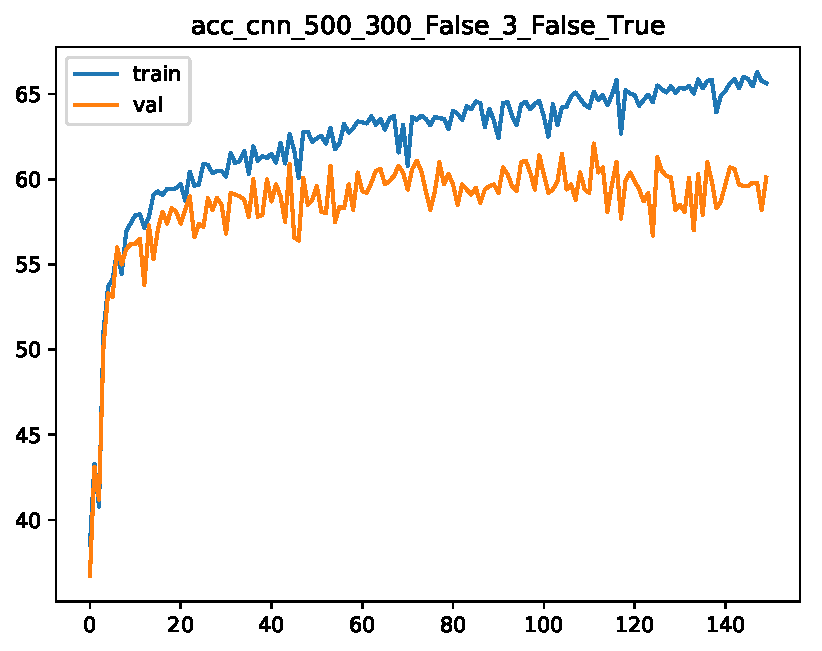
\includegraphics[width = 2.5cm]{acc_cnn_500_300_False_3_False_True.pdf}
}	
\subfloat[300 RNN]{
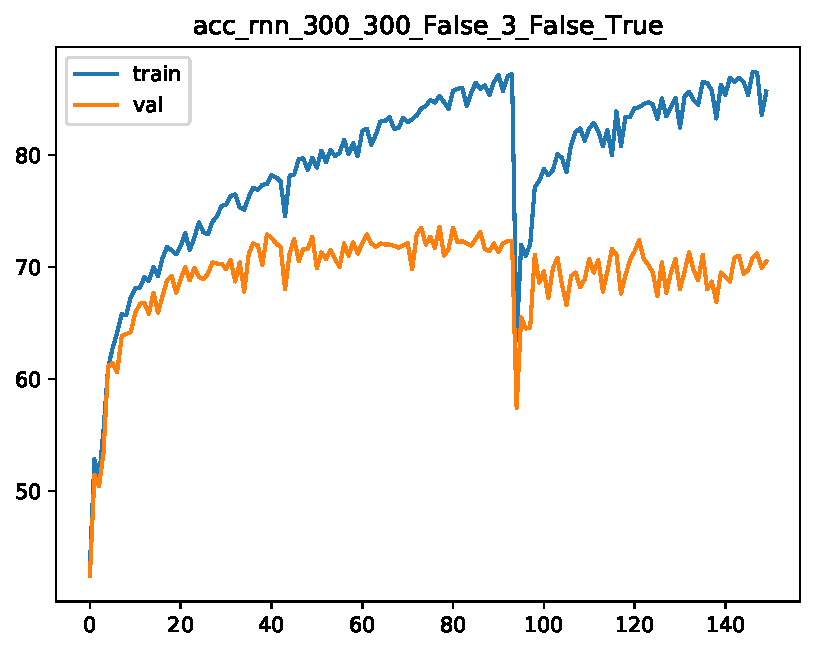
\includegraphics[width = 2.5cm]{acc_rnn_300_300_False_3_False_True.pdf}
}
\subfloat[400 RNN]{
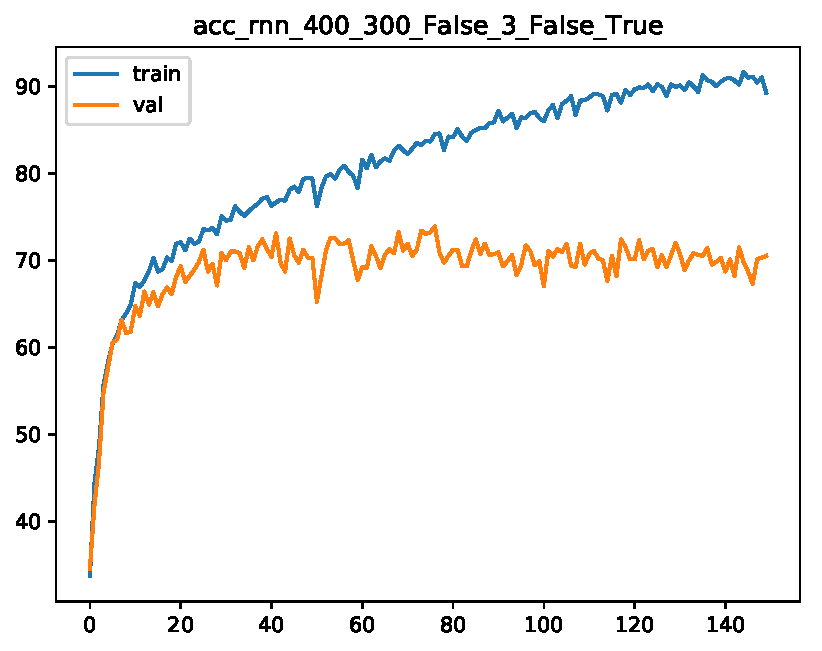
\includegraphics[width = 2.5cm]{acc_rnn_400_300_False_3_False_True.pdf}
}	
\subfloat[500 RNN]{
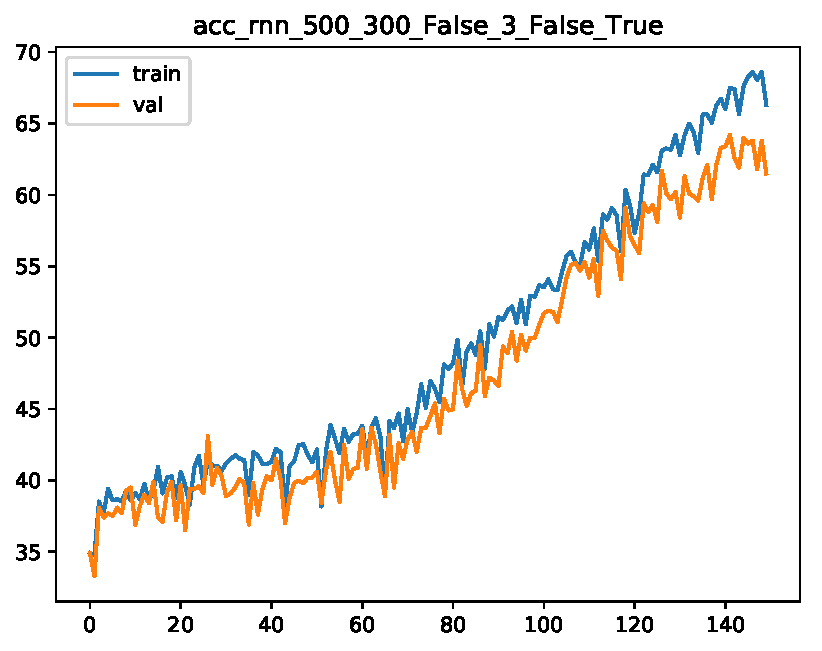
\includegraphics[width = 2.5cm]{acc_rnn_500_300_False_3_False_True.pdf}
}\\
\subfloat[300 CNN]{
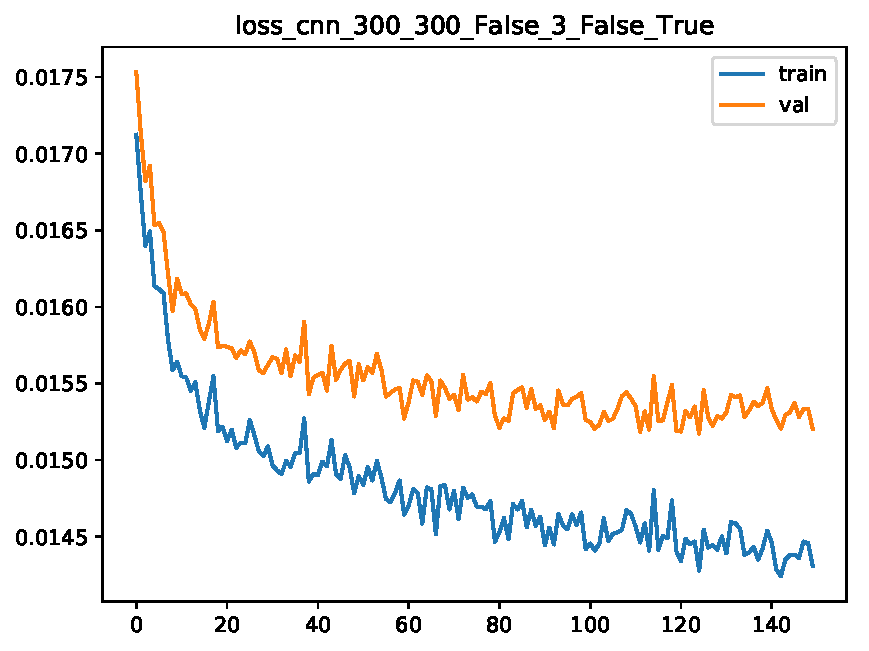
\includegraphics[width = 2.5cm]{loss_cnn_300_300_False_3_False_True.pdf}
}
\subfloat[400 CNN]{
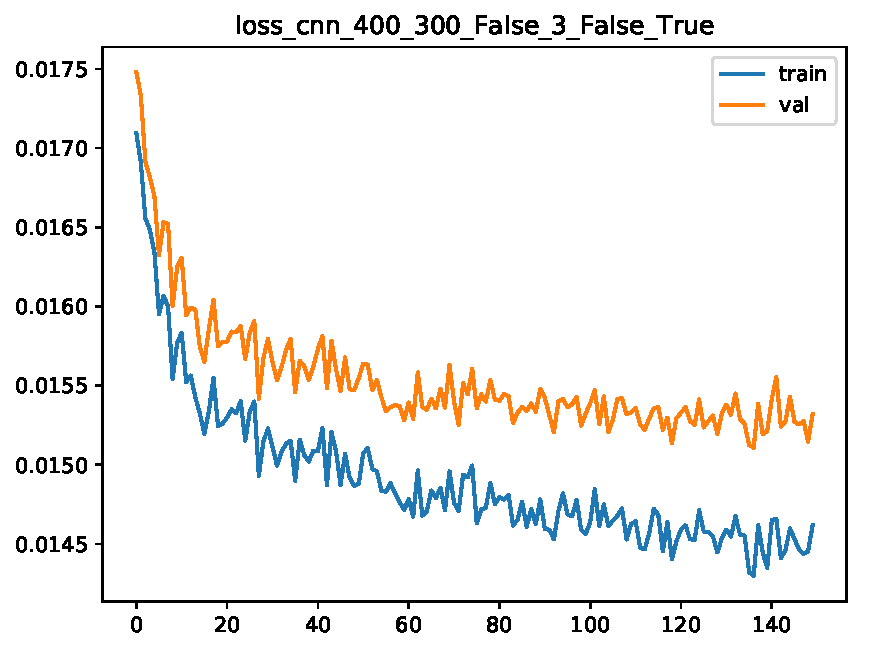
\includegraphics[width = 2.5cm]{loss_cnn_400_300_False_3_False_True.pdf}
}	
\subfloat[500 CNN]{
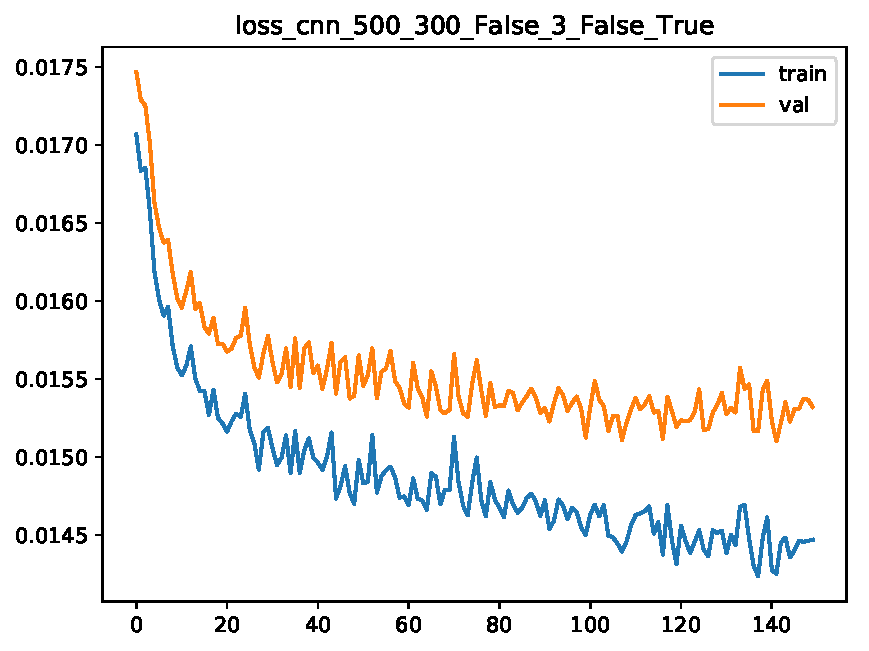
\includegraphics[width = 2.5cm]{loss_cnn_500_300_False_3_False_True.pdf}
}	
\subfloat[300 RNN]{
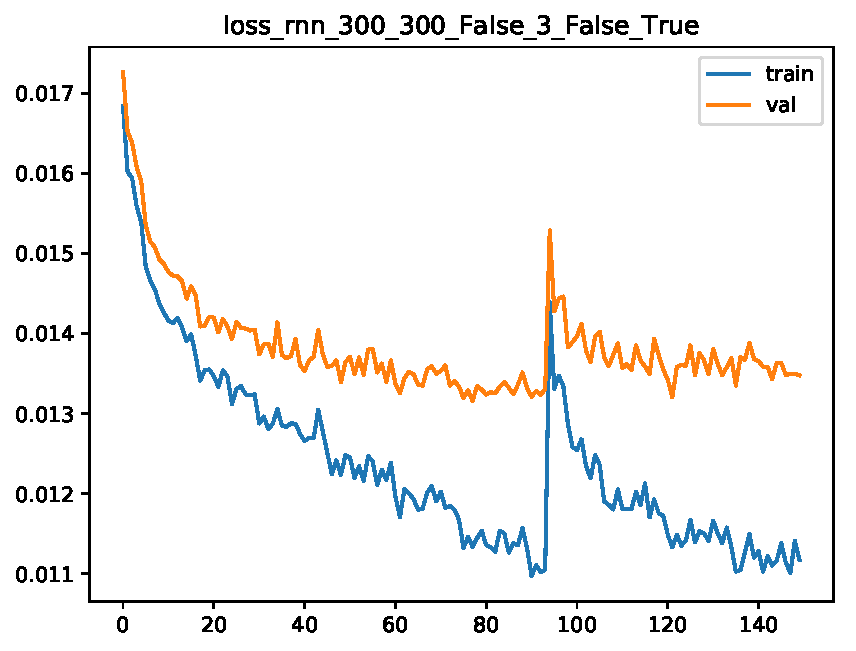
\includegraphics[width = 2.5cm]{loss_rnn_300_300_False_3_False_True.pdf}
}
\subfloat[400 RNN]{
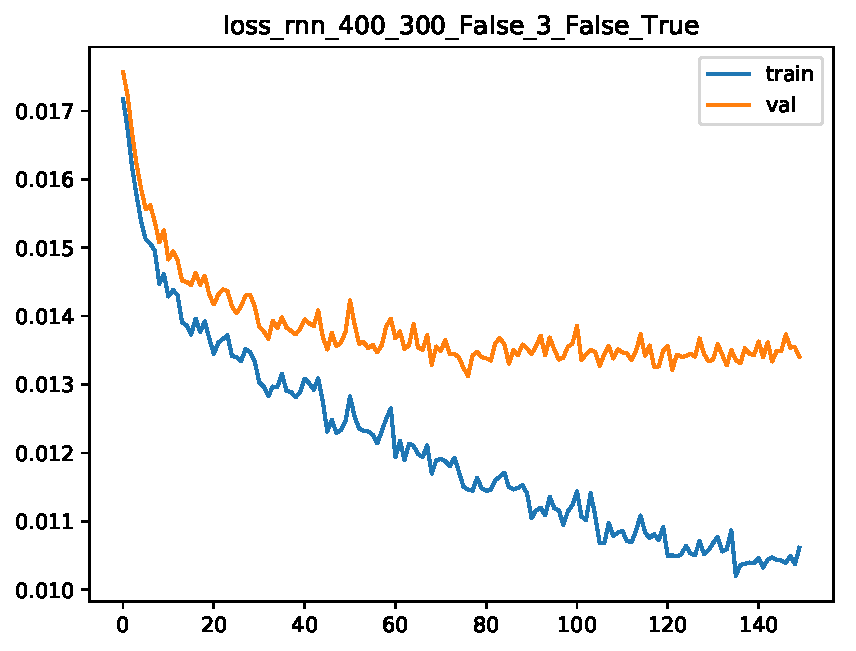
\includegraphics[width = 2.5cm]{loss_rnn_400_300_False_3_False_True.pdf}
}	
\subfloat[500 RNN]{
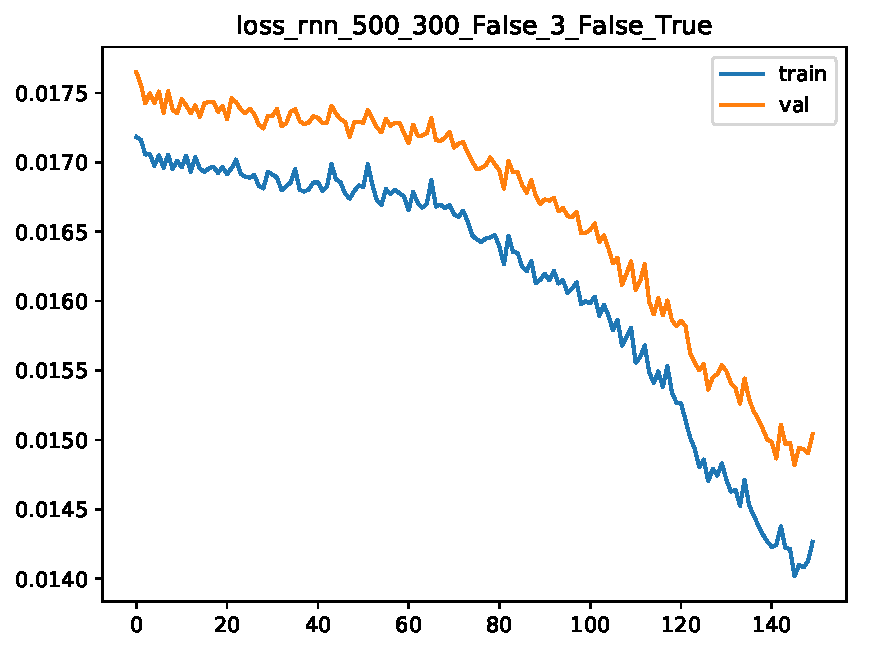
\includegraphics[width = 2.5cm]{loss_rnn_500_300_False_3_False_True.pdf}
}
\caption{\label{fig: hid}Accuracy and Loss on Validation and Train Set When We Vary Hidden Sizes, and Fix the Others.}
\end{figure}
 
\subsection{Vary Kernel Size}
We use the previously tuned best \texttt{hidden\_size} = 300 and vary kernel size only for CNN. The results are shown in Table \ref{tab: kernel} and Figure \ref{fig: kernel}. The best kernel size is 3. Usually, small kernel size catches high frequency features. Here, maybe high frequency features are more important. Another view is that kernel size 3 is corresponding to 3-gram and kernel size 5 is corresponding to 5-gram. 3-gram may play a more important part in SNLI classification. Actually, the accuracy is very close so kernel size does not matter too much.
\begin{table}[!ht]
\centering
\begin{tabular}{|c|c|c|}
\hline
kernel size & 3 & 5\\ \hline
Validation Accuracy & \textbf{62.3} & 60.7\\ \hline
number of parameters & 632103 & 992103 \\ \hline
\end{tabular}
\caption{\label{tab: kernel}Accuracy on Validation Set and Number of Parameters When We Vary Kernel Sizes, and Fix the Others.}
\end{table}
\begin{figure}[!ht]
\centering
\subfloat[3]{
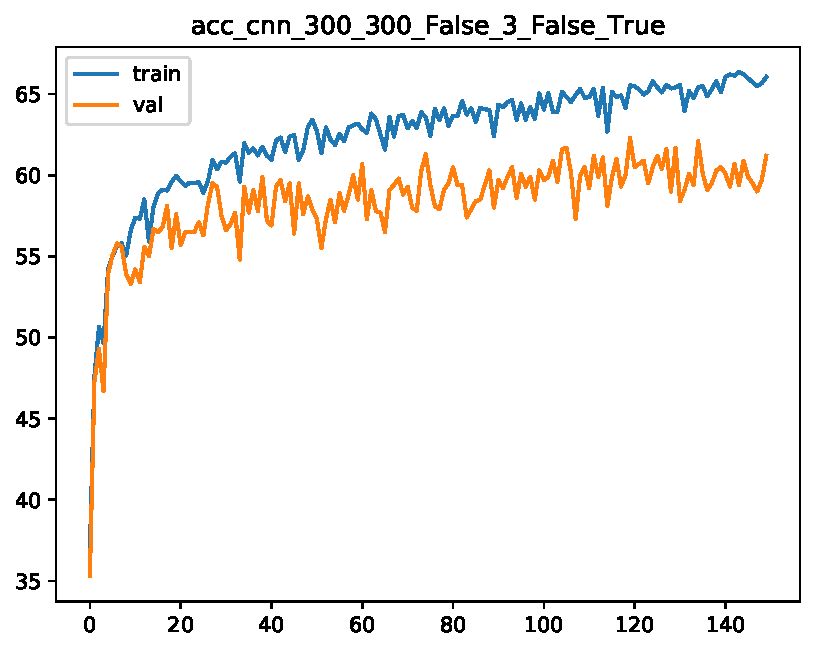
\includegraphics[width = 2.5cm]{acc_cnn_300_300_False_3_False_True.pdf}
}
\subfloat[3]{
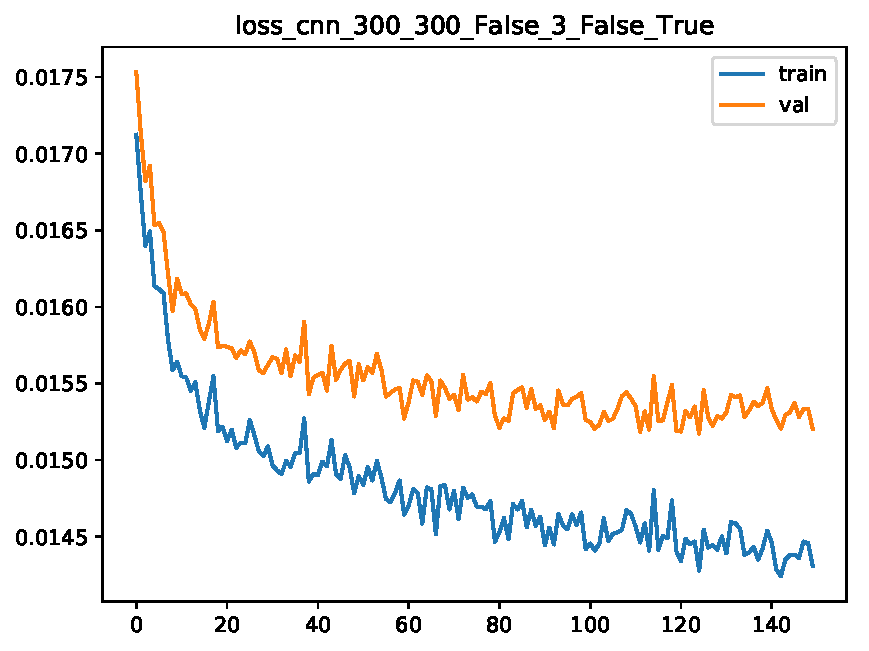
\includegraphics[width = 2.5cm]{loss_cnn_300_300_False_3_False_True.pdf}
}	
\subfloat[5]{
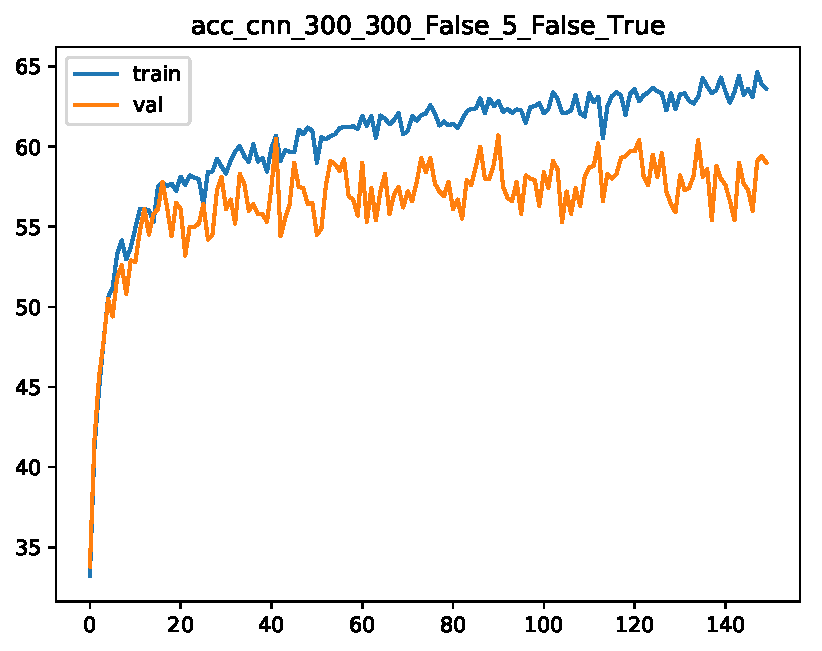
\includegraphics[width = 2.5cm]{acc_cnn_300_300_False_5_False_True.pdf}
}	
\subfloat[5]{
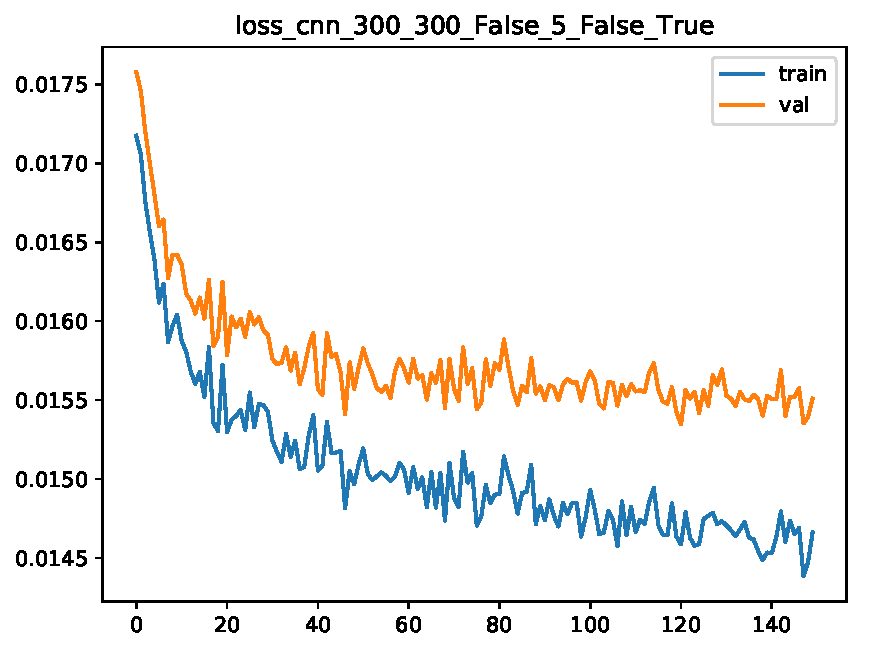
\includegraphics[width = 2.5cm]{loss_cnn_300_300_False_5_False_True.pdf}
}	
\caption{\label{fig: kernel}Accuracy and Loss on Validation and Train Set When We Vary Kernel Sizes, and Fix the Others.}
\end{figure}

\subsection{Concatenation or Element-wise Multiplication}
We choose hidden size 300 and kernel size 3 for CNN and hidden size 400 for RNN. We vary the way of combining two representations after encoding. The results are shown in Table \ref{tab: comb} and Figure \ref{fig: comb}. We find that CNN prefers concatenation and RNN prefers element-wise multiplication. In GRU, we some sense of multiplication between features through gates. Maybe this makes RNN prefers multiplication. It is hard to say why one way of combining representations is better than the other.
\begin{table}[!ht]
\centering
\begin{tabular}{|c|c|c|c|c|}
\hline
Network & \multicolumn{2}{|c|}{CNN} & \multicolumn{2}{|c|}{RNN} \\ \hline
Combining Method & Concatenation & Element-wise Multiplication & Concatenation & Element-wise Multiplication \\ \hline
Validation Accuracy & \textbf{64.6} & 62.3 & 66.7 & \textbf{73.9}\\ \hline
number of parameters & 722103 & 632103 & 1926303 &1806303 \\ \hline
\end{tabular}
\caption{\label{tab: comb}Accuracy on Validation Set and Number of Parameters When We Vary Combining Methods, and Fix the Others.}
\end{table}
\begin{figure}[!ht]
\centering
\subfloat[False, CNN]{
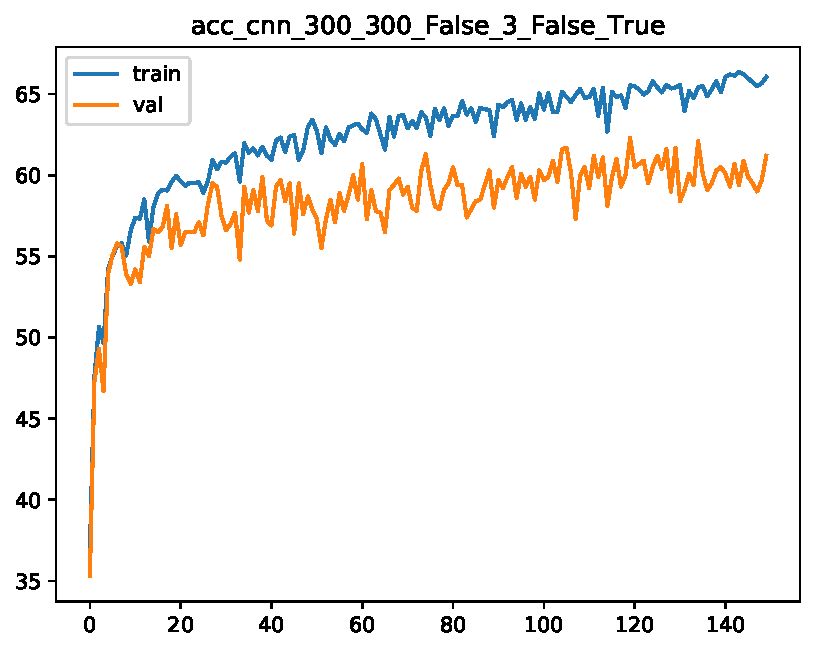
\includegraphics[width = 2.5cm]{acc_cnn_300_300_False_3_False_True.pdf}
}
\subfloat[False, CNN]{
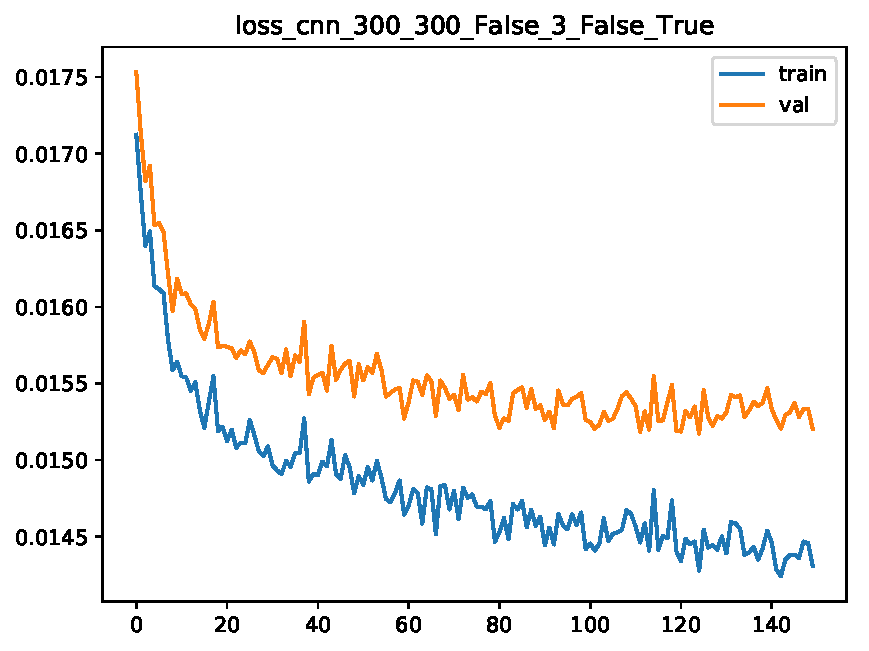
\includegraphics[width = 2.5cm]{loss_cnn_300_300_False_3_False_True.pdf}
}	
\subfloat[True, CNN]{
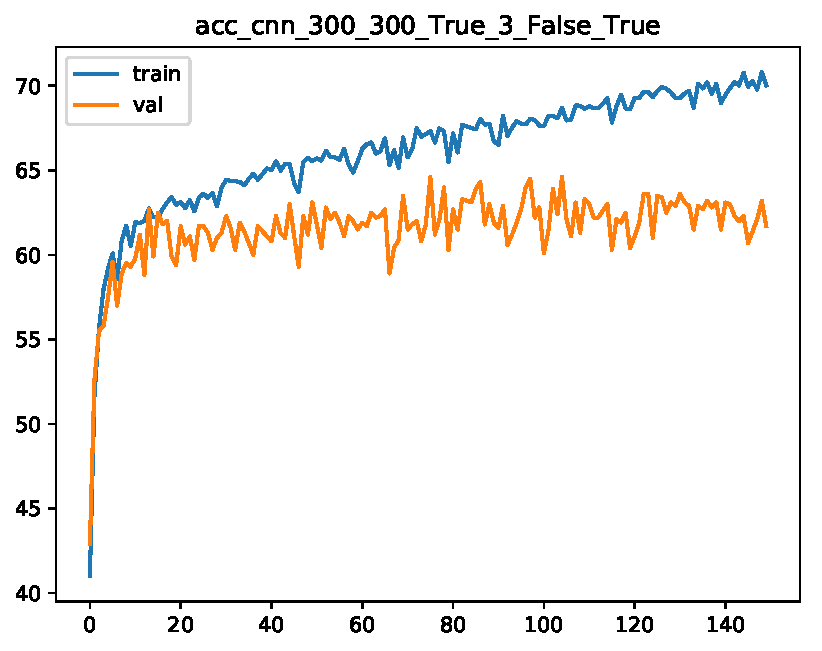
\includegraphics[width = 2.5cm]{acc_cnn_300_300_True_3_False_True.pdf}
}
\subfloat[True, CNN]{
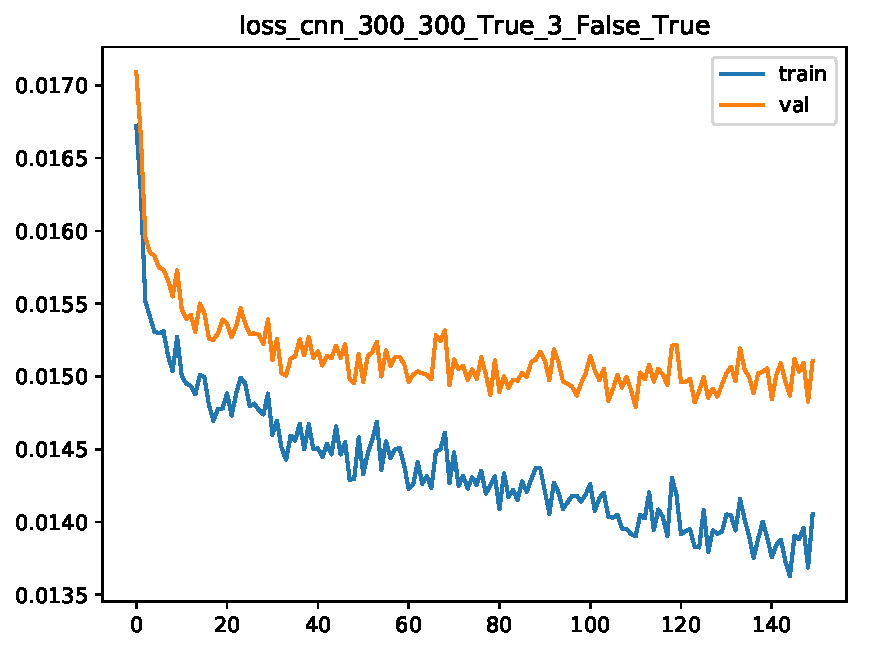
\includegraphics[width = 2.5cm]{loss_cnn_300_300_True_3_False_True.pdf}
}	\\
\subfloat[False, RNN]{
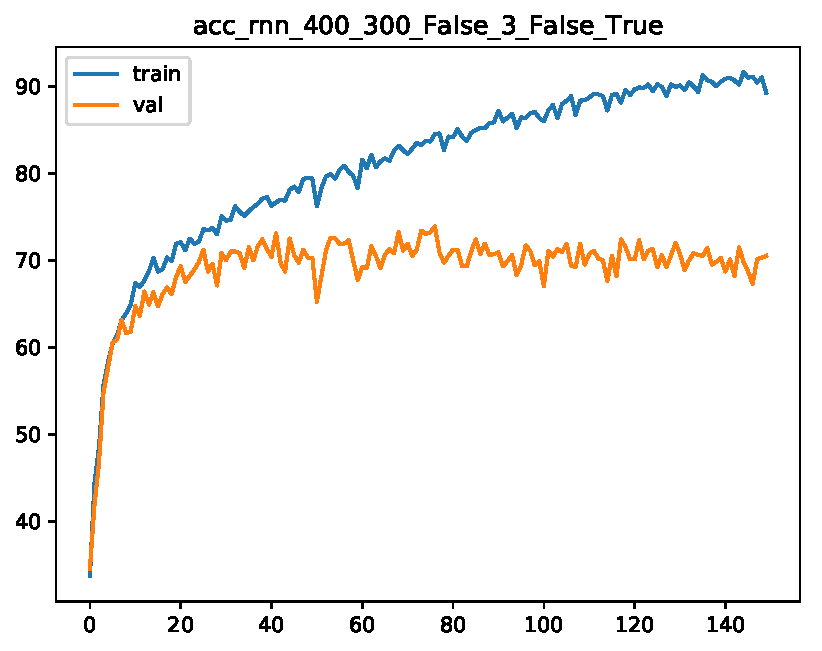
\includegraphics[width = 2.5cm]{acc_rnn_400_300_False_3_False_True.pdf}
}
\subfloat[False, RNN]{
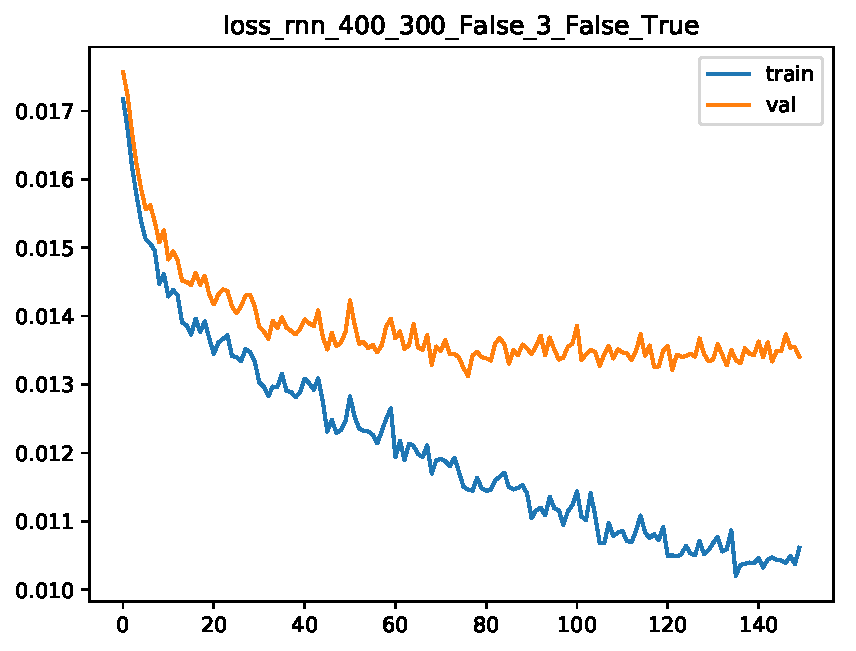
\includegraphics[width = 2.5cm]{loss_rnn_400_300_False_3_False_True.pdf}
}	
\subfloat[True, RNN]{
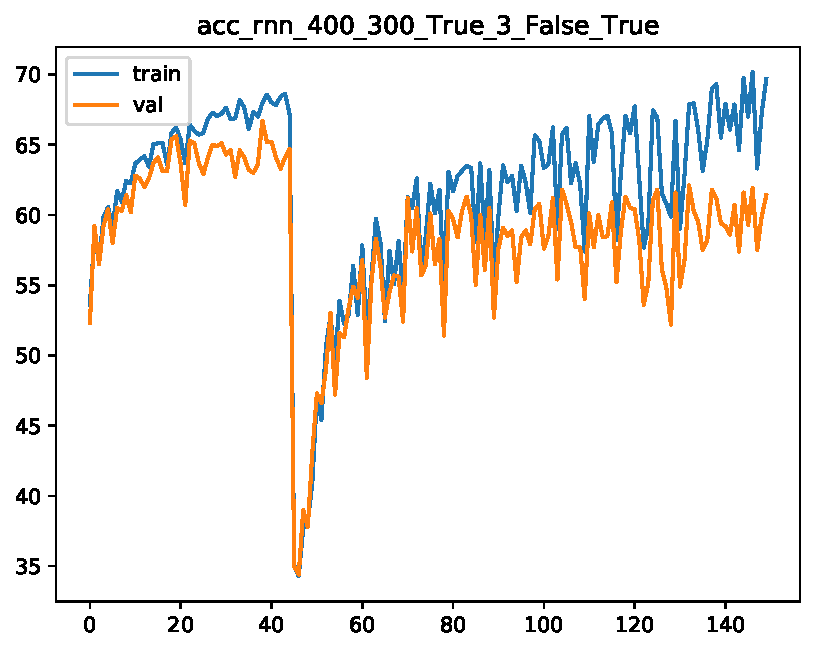
\includegraphics[width = 2.5cm]{acc_rnn_400_300_True_3_False_True.pdf}
}
\subfloat[True, RNN]{
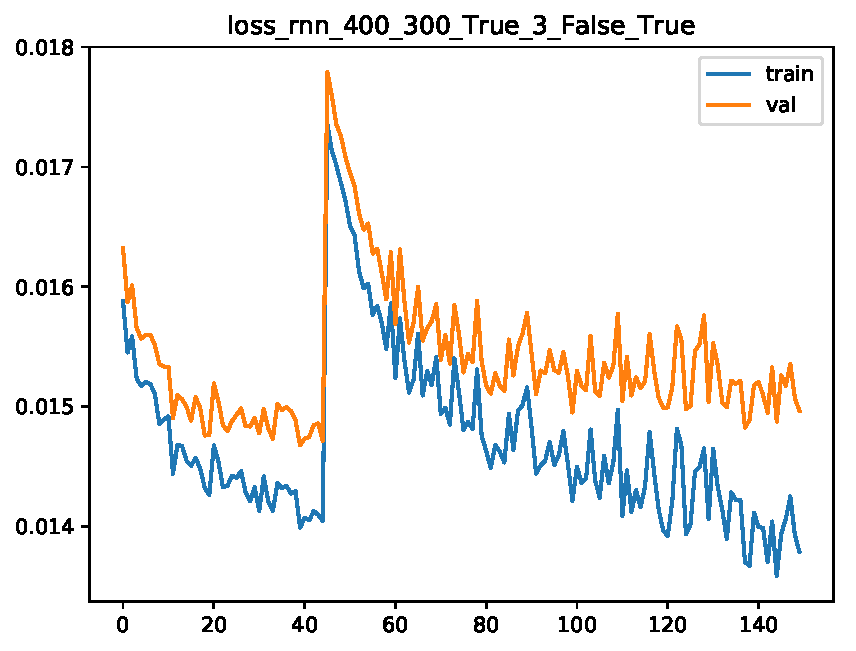
\includegraphics[width = 2.5cm]{loss_rnn_400_300_True_3_False_True.pdf}
}	
\caption{\label{fig: comb}Accuracy and Loss on Validation and Train Set When We Vary Combining Methods, and Fix the Others.}
\end{figure}
\subsection{Vary Regularizations}
We use weight decay = 5e-4 in Adam and a dropout layer between two fully connected layers. The results are in Table \ref{tab: reg} and Figure \ref{fig: reg}. Weight decay does not work for this task. The reason could be the penalty level is too high or the same learning rate does not work for weight decay. To be honest, I do not have time to explore learning rate and weight decay. Dropout is better for RNN but not for CNN. For CNN, the difference of validation accuracy for with dropout and without dropout is very small, like 0.4. So we could not make a strong conclusion that dropout does not work here.
\begin{table}[!ht]
\centering
\begin{tabular}{|c|c|c|c|c|c|c|c|c|}
\hline
Network & \multicolumn{4}{|c|}{CNN} & \multicolumn{4}{|c|}{RNN} \\ \hline
\texttt{is\_dropout} & \multicolumn{2}{|c|}{True}& \multicolumn{2}{|c|}{False}& \multicolumn{2}{|c|}{True} & \multicolumn{2}{|c|}{False}\\ \hline
\texttt{is\_wd} & True& False & True& False & True& False& True& False\\ \hline
validation accuracy & 37.7 &  64.6 & 40.5 & \textbf{65.0} & 36.0 & \textbf{73.9} & 35.3 & 67.8\\ \hline
number of parameters & 722103 & 722103 & 722103 &722103 & 1806303 & 1806303 & 1806303&1806303\\ \hline
\end{tabular}
\caption{\label{tab: reg}Accuracy on Validation Set and Number of Parameters When We Vary Combining Methods, and Fix the Others.}
\end{table}
\begin{figure}[!ht]
\centering
\subfloat[False, True, CNN]{
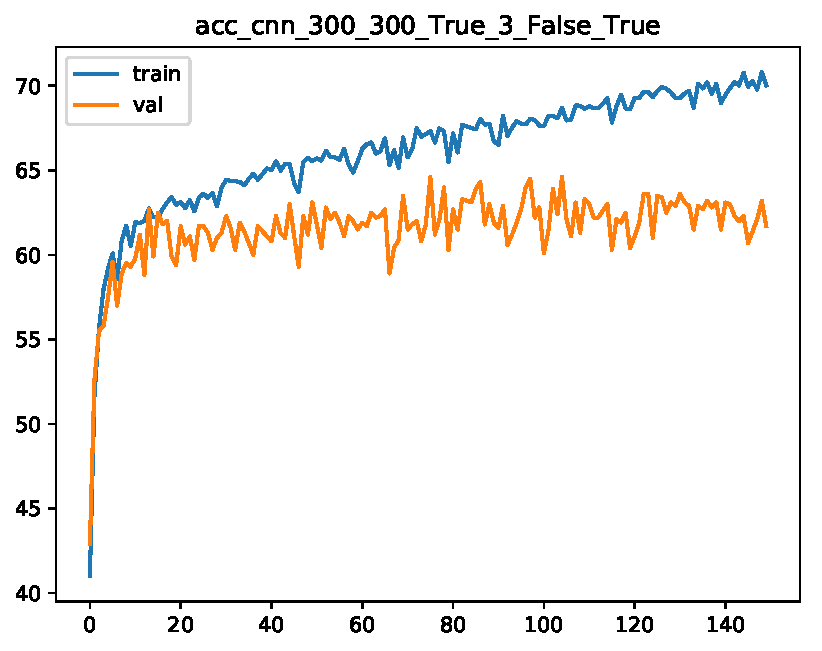
\includegraphics[width = 2.5cm]{acc_cnn_300_300_True_3_False_True.pdf}
}
\subfloat[False, True, CNN]{
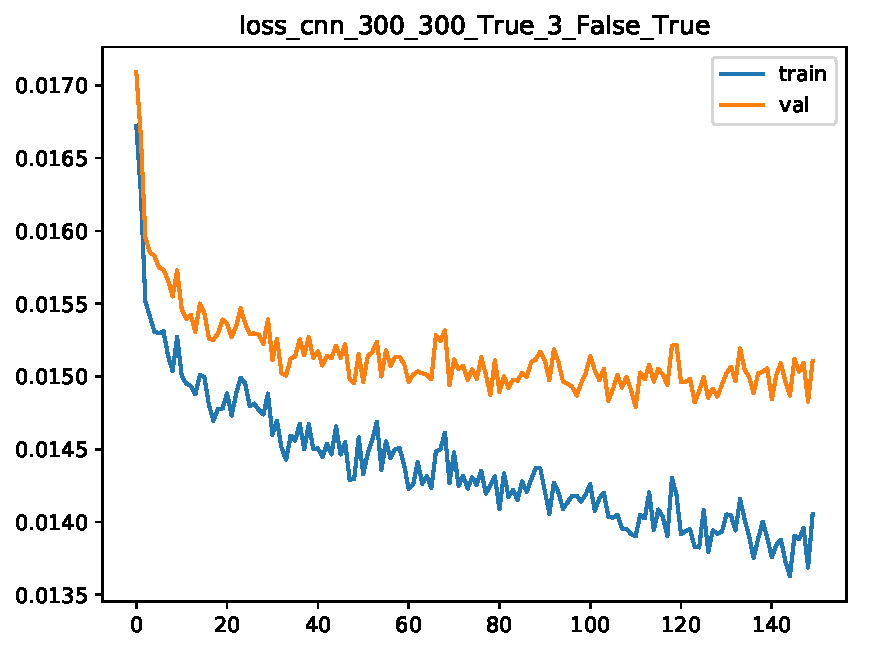
\includegraphics[width = 2.5cm]{loss_cnn_300_300_True_3_False_True.pdf}
}	
\subfloat[False, False, CNN]{
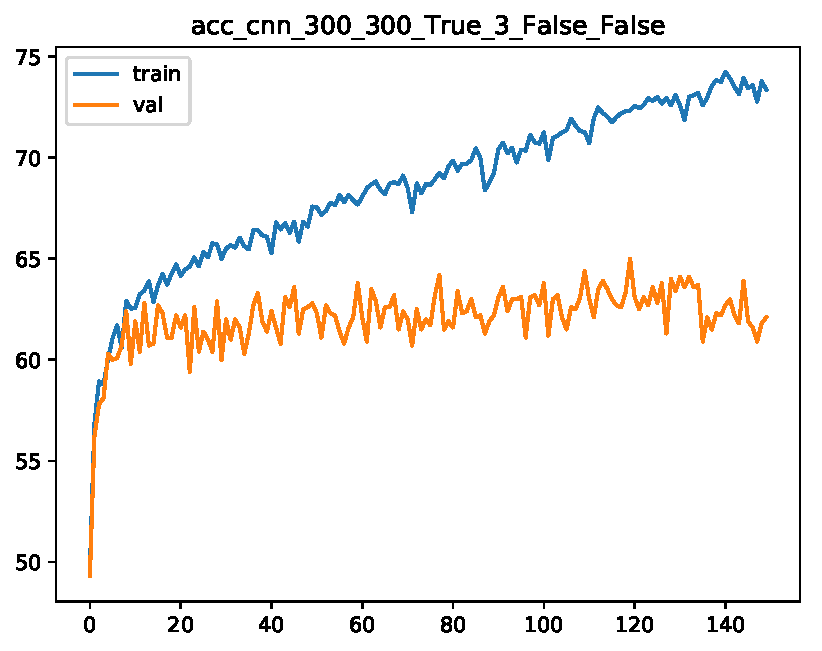
\includegraphics[width = 2.5cm]{acc_cnn_300_300_True_3_False_False.pdf}
}
\subfloat[False, False, CNN]{
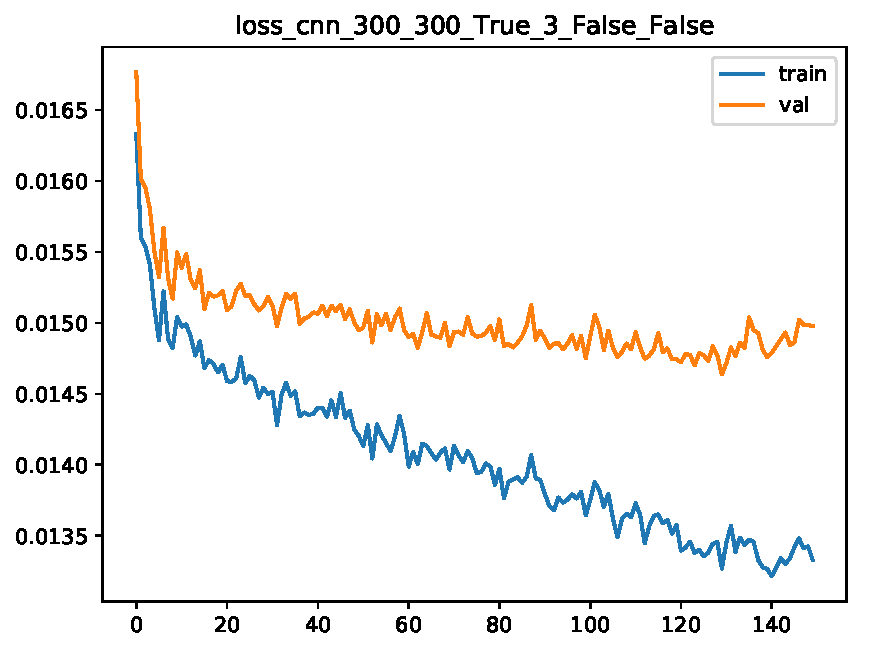
\includegraphics[width = 2.5cm]{loss_cnn_300_300_True_3_False_False.pdf}
}	
\subfloat[True, False, CNN]{
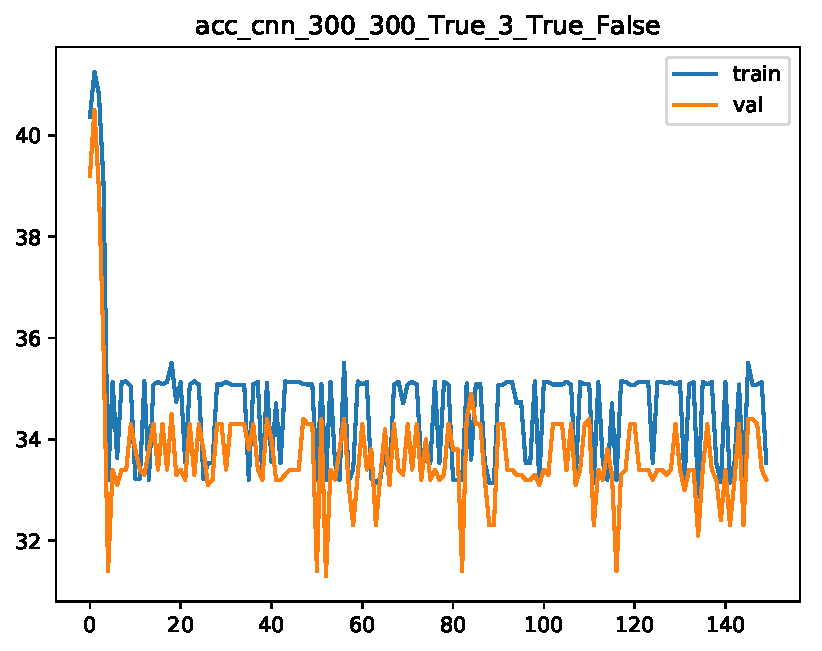
\includegraphics[width = 2.5cm]{acc_cnn_300_300_True_3_True_False.pdf}
}
\subfloat[True, False, CNN]{
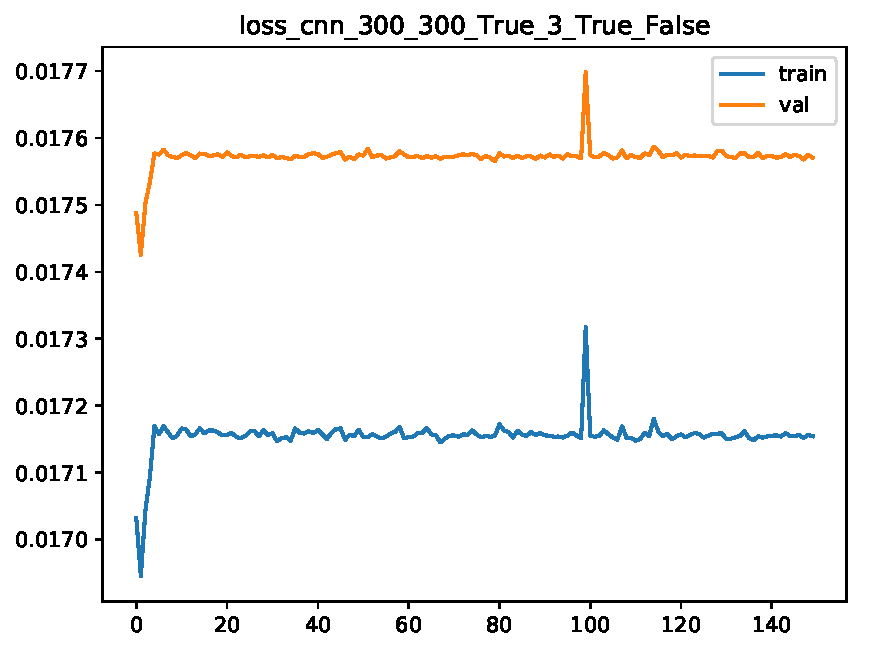
\includegraphics[width = 2.5cm]{loss_cnn_300_300_True_3_True_False.pdf}
}	\\
\subfloat[True, True, CNN]{
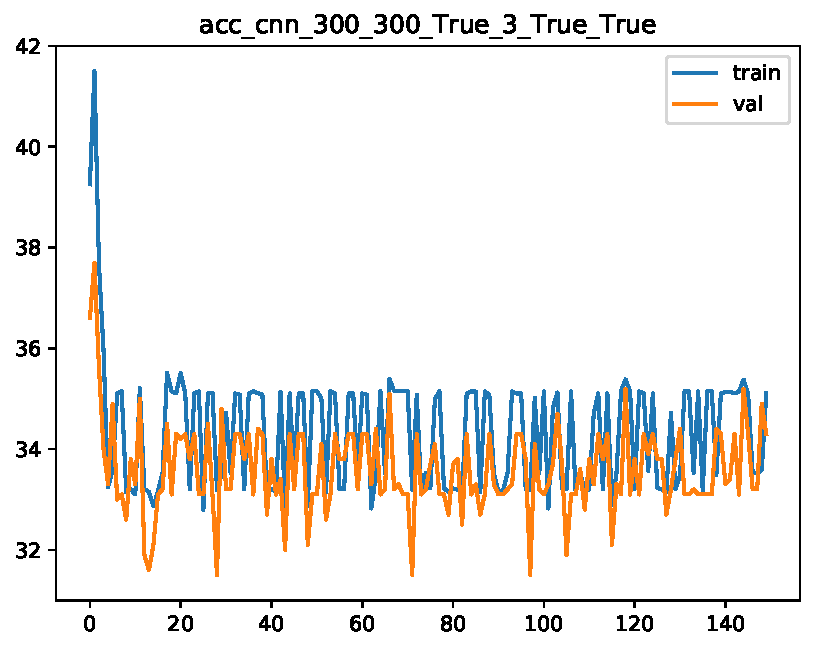
\includegraphics[width = 2.5cm]{acc_cnn_300_300_True_3_True_True.pdf}
}
\subfloat[True, True, CNN]{
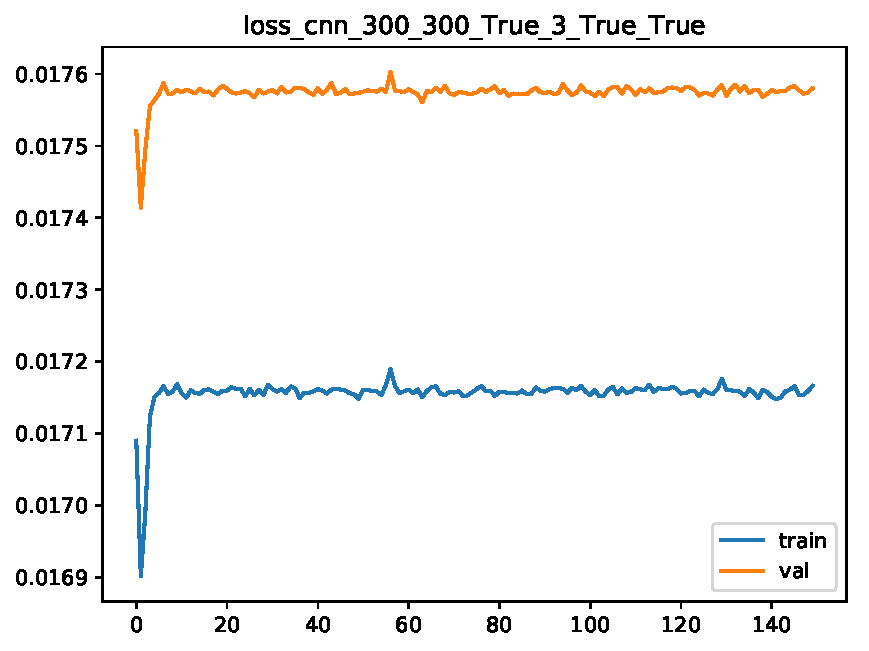
\includegraphics[width = 2.5cm]{loss_cnn_300_300_True_3_True_True.pdf}
}	
\subfloat[False, True, RNN]{
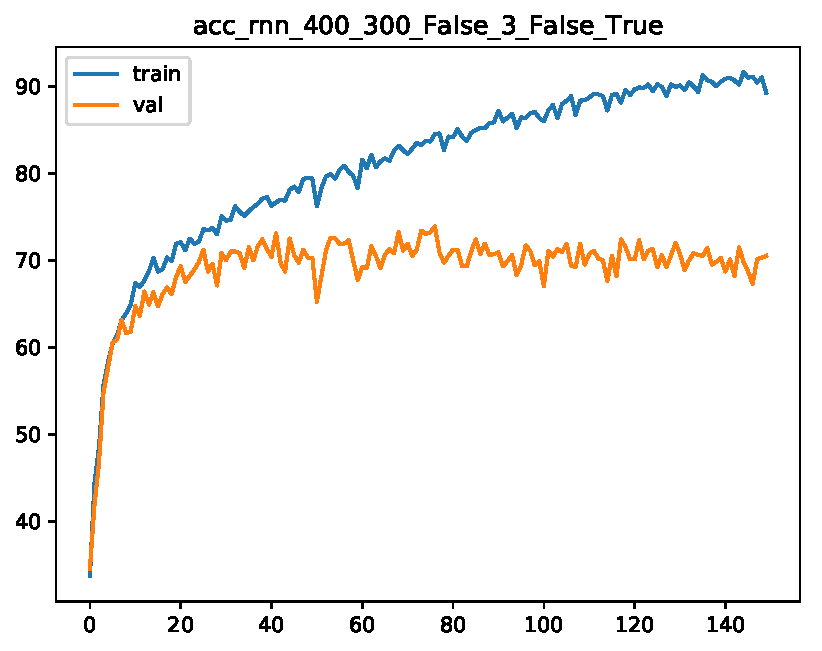
\includegraphics[width = 2.5cm]{acc_rnn_400_300_False_3_False_True.pdf}
}
\subfloat[False, True, RNN]{
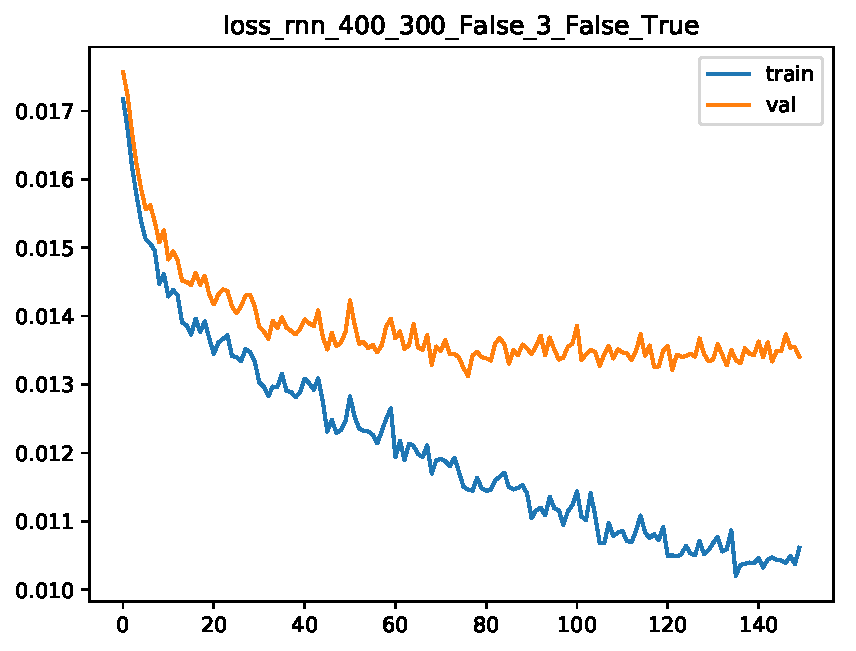
\includegraphics[width = 2.5cm]{loss_rnn_400_300_False_3_False_True.pdf}
}	
\subfloat[False, False, RNN]{
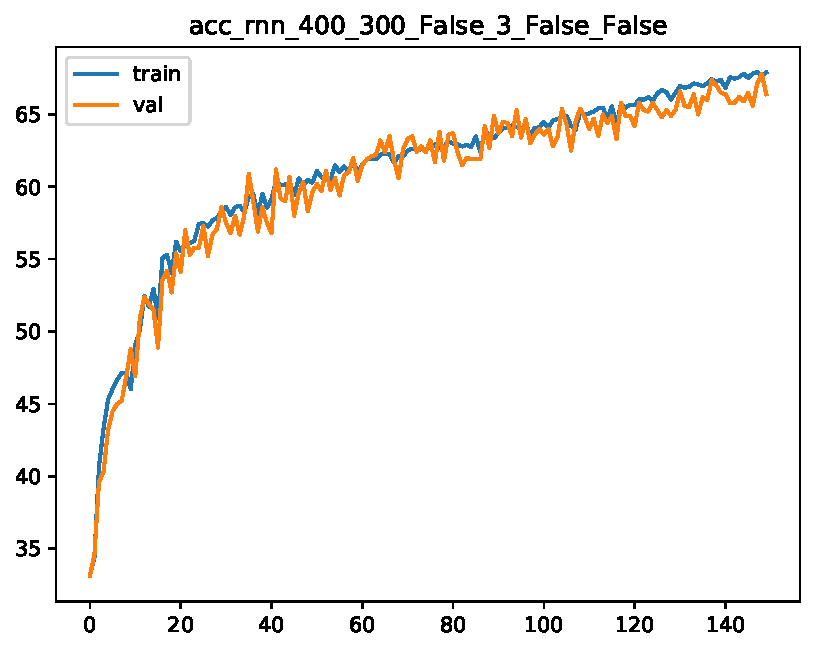
\includegraphics[width = 2.5cm]{acc_rnn_400_300_False_3_False_False.pdf}
}
\subfloat[False, False, RNN]{
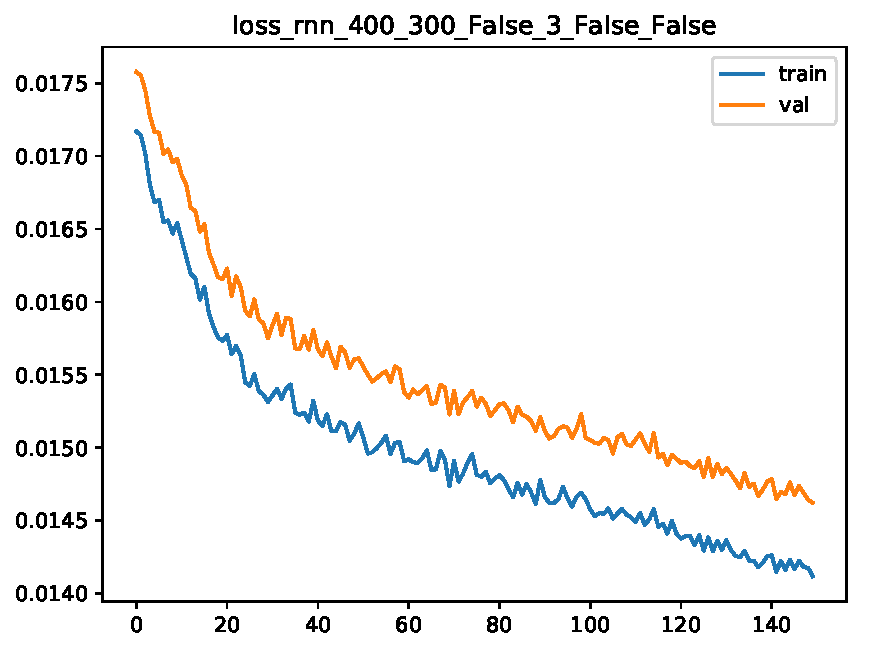
\includegraphics[width = 2.5cm]{loss_rnn_400_300_False_3_False_False.pdf}
}	\\
\subfloat[True, False, RNN]{
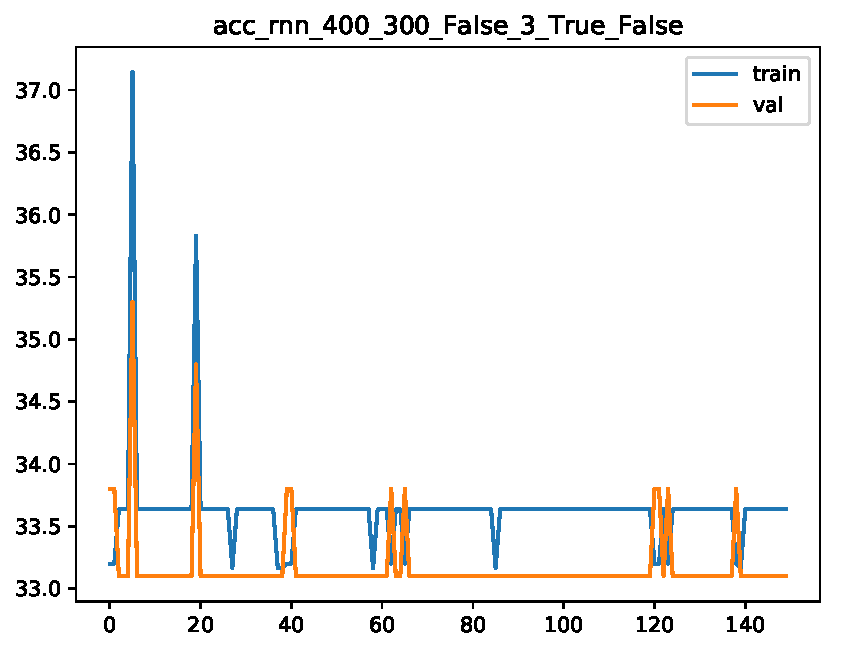
\includegraphics[width = 2.5cm]{acc_rnn_400_300_False_3_True_False.pdf}
}
\subfloat[True, False, RNN]{
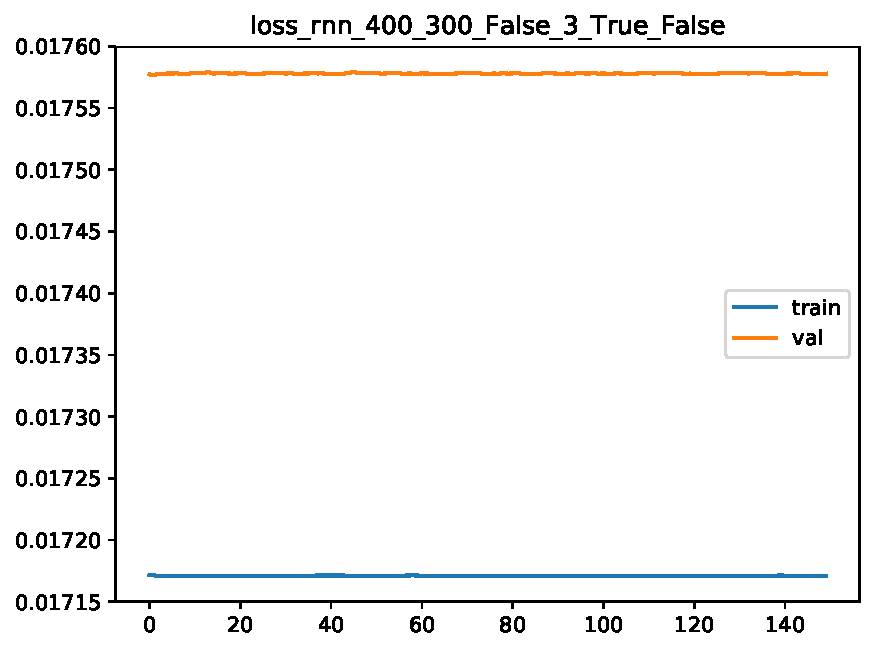
\includegraphics[width = 2.5cm]{loss_rnn_400_300_False_3_True_False.pdf}
}	
\subfloat[True, True, RNN]{
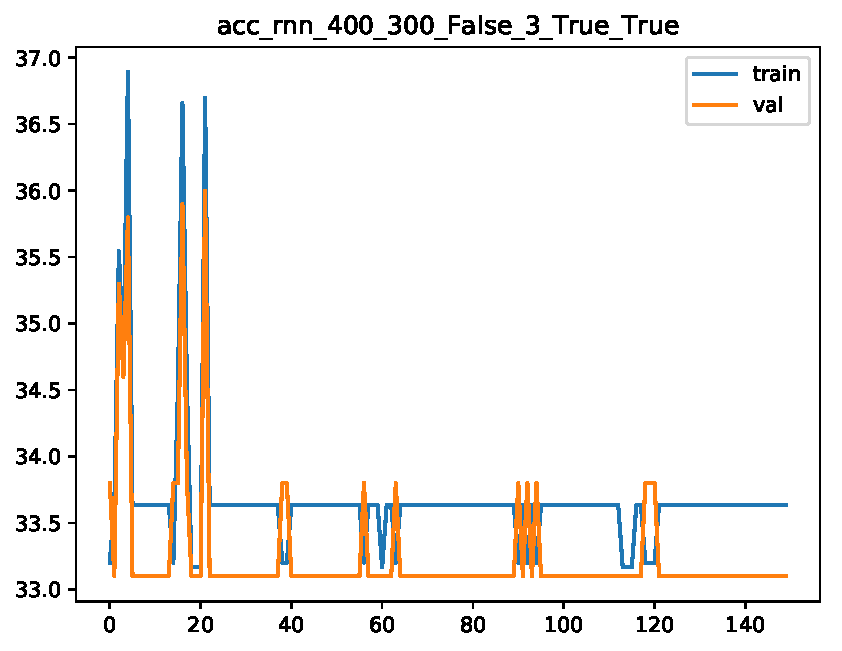
\includegraphics[width = 2.5cm]{acc_rnn_400_300_False_3_True_True.pdf}
}
\subfloat[True, True, RNN]{
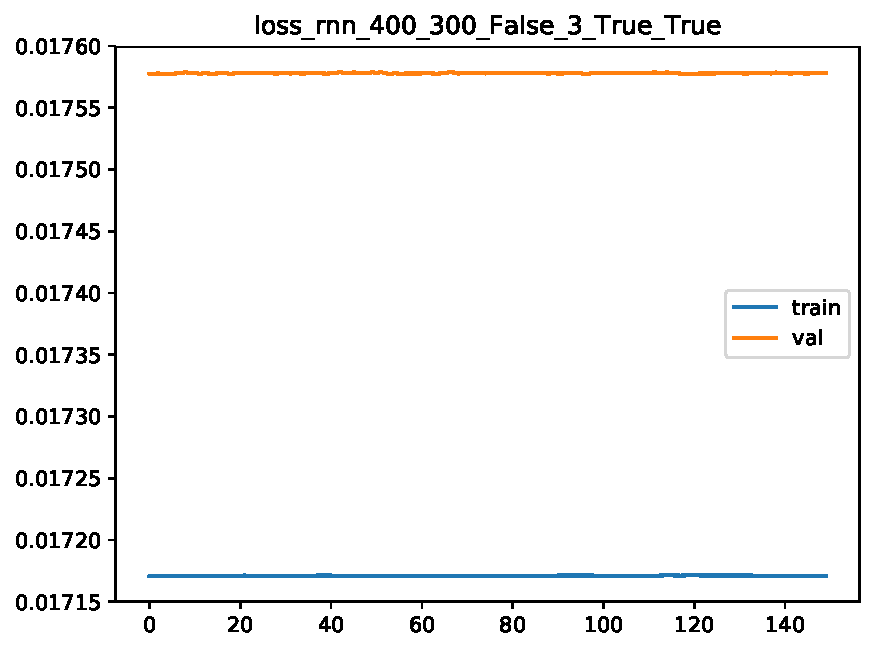
\includegraphics[width = 2.5cm]{loss_rnn_400_300_False_3_True_True.pdf}
}	
\caption{\label{fig: reg}Accuracy and Loss on Validation and Train Set When We Vary Regularization Methods, and Fix the Others.}
\end{figure}
%\begin{figure}[!ht]
%\centering
%\subfloat[(Adam,F,0.001)]{
%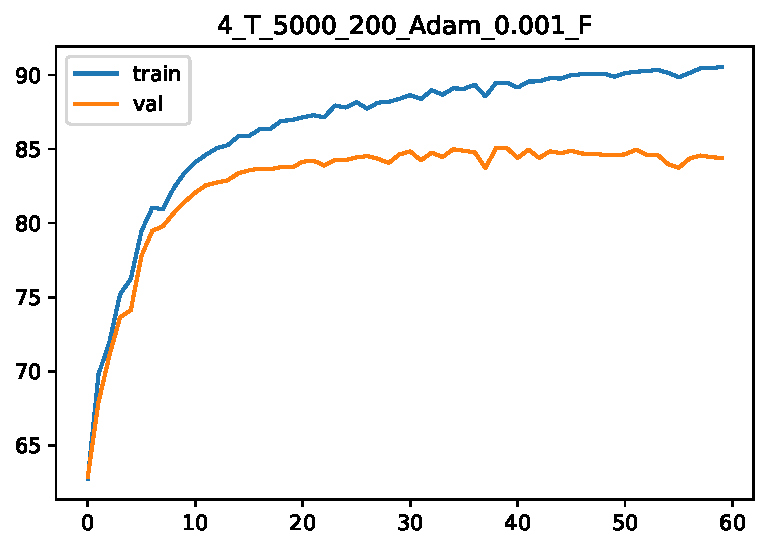
\includegraphics[width = 3cm]{4_T_5000_200_Adam_0001_F.pdf}
%}
%\subfloat[(Adam,T,0.001)]{
%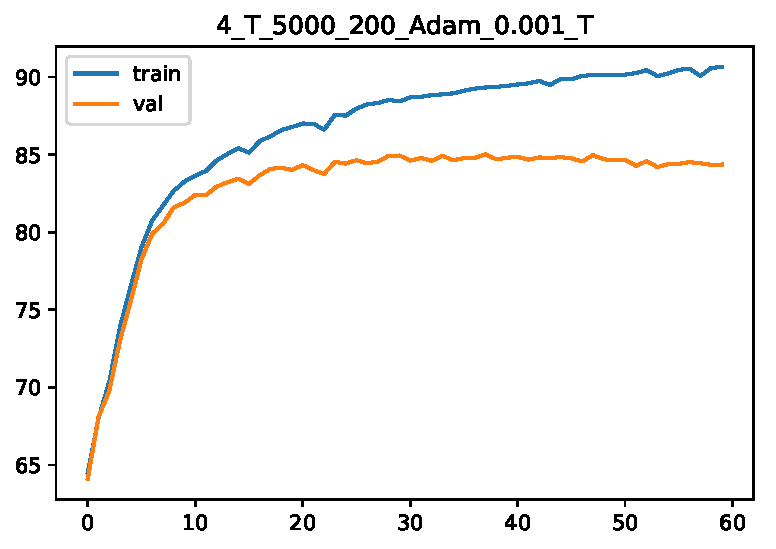
\includegraphics[width = 3cm]{4_T_5000_200_Adam_0001_T.pdf}
%}	
%\subfloat[(SGD,F,0.001)]{
%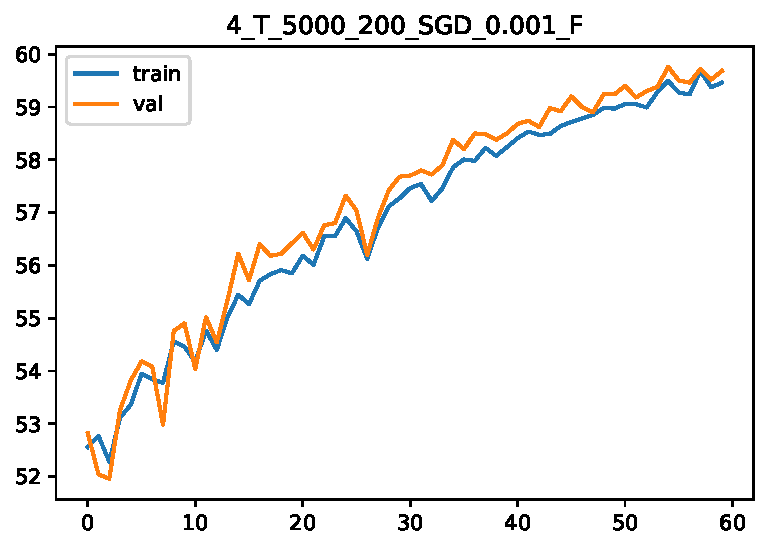
\includegraphics[width = 3cm]{4_T_5000_200_SGD_0001_F.pdf}
%}
%\subfloat[(SGD,T,0.001)]{
%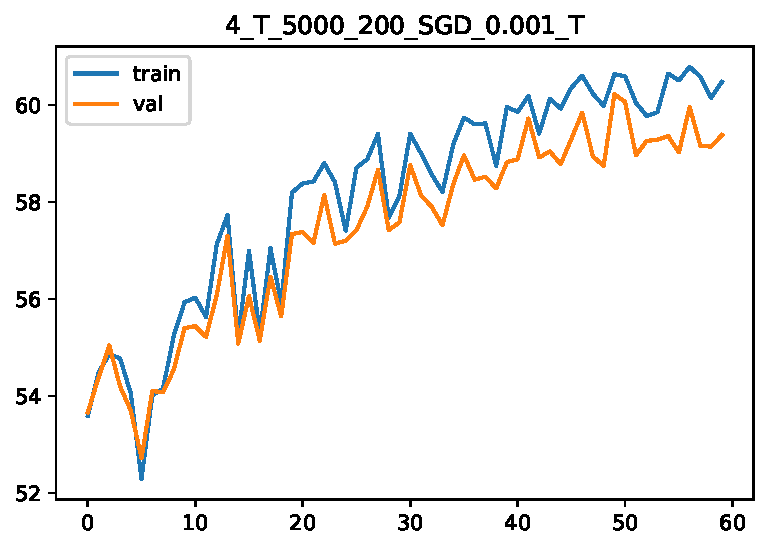
\includegraphics[width = 3cm]{4_T_5000_200_SGD_0001_T.pdf}
%}		\\
%\subfloat[(Adam,F,0.01)]{
%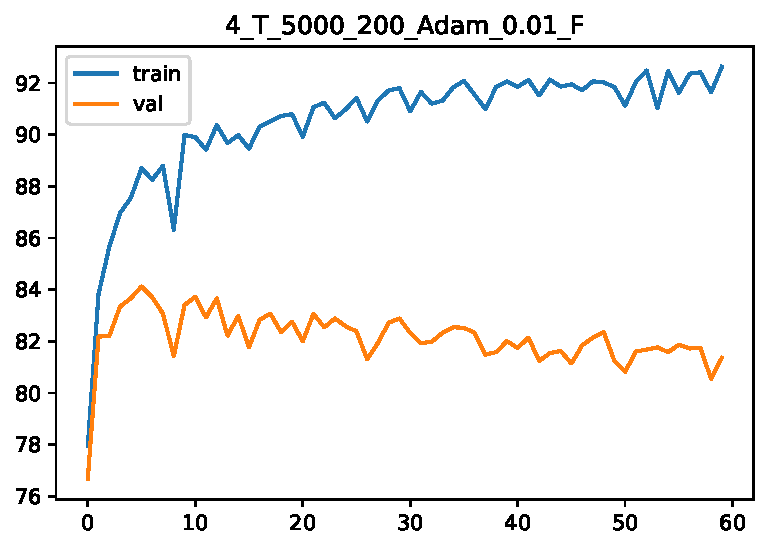
\includegraphics[width = 3cm]{4_T_5000_200_Adam_001_F.pdf}
%}
%\subfloat[(Adam,T,0.01)]{
%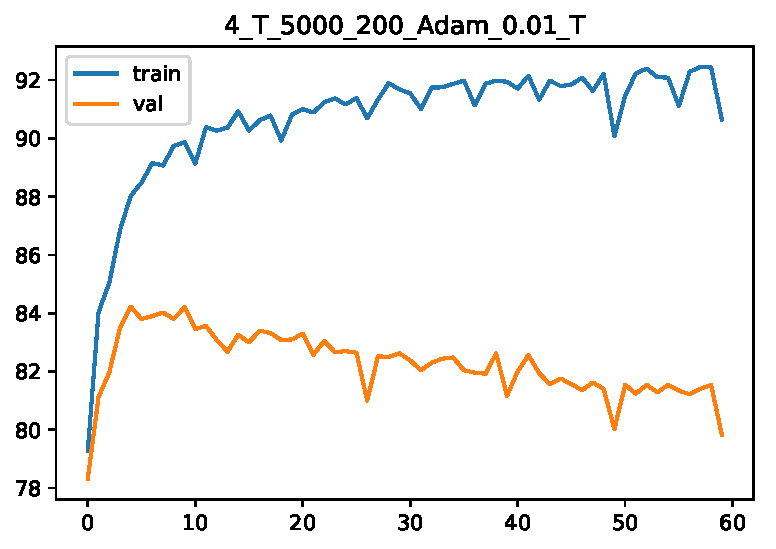
\includegraphics[width = 3cm]{4_T_5000_200_Adam_001_T.pdf}
%}	
%\subfloat[(SGD,F,0.01)]{
%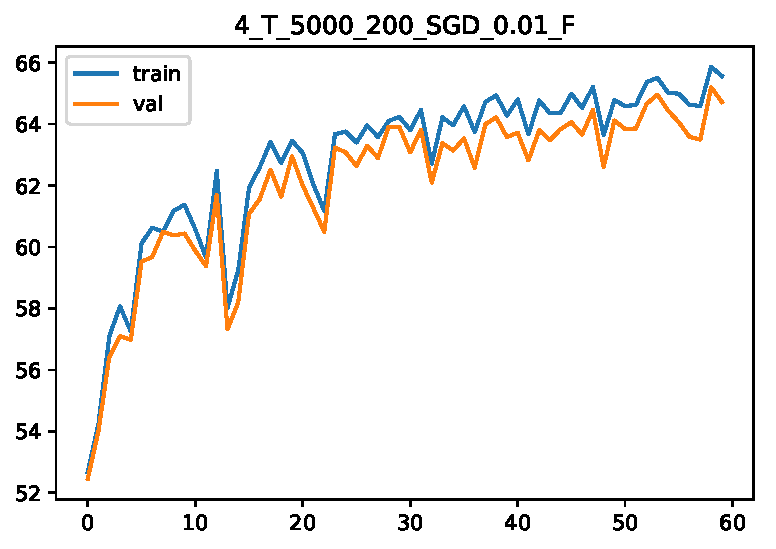
\includegraphics[width = 3cm]{4_T_5000_200_SGD_001_F.pdf}
%}
%\subfloat[(SGD,T,0.01)]{
%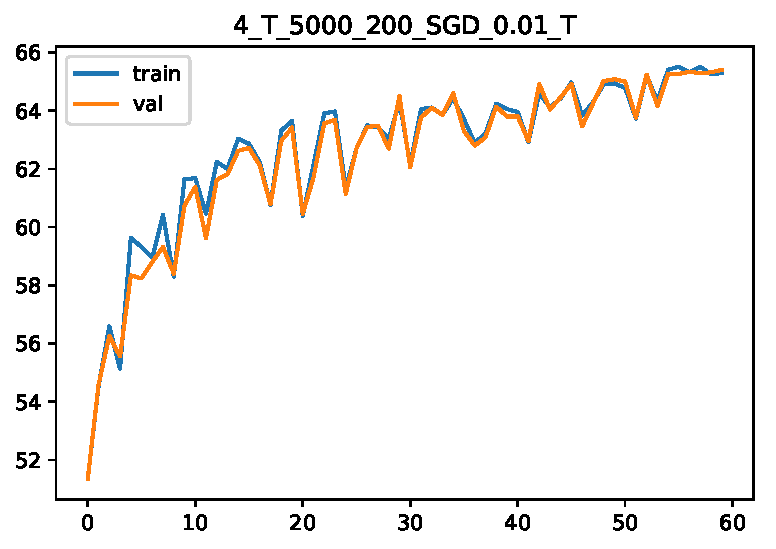
\includegraphics[width = 3cm]{4_T_5000_200_SGD_001_T.pdf}
%}		\\
%\subfloat[(Adam,F,0.1)]{
%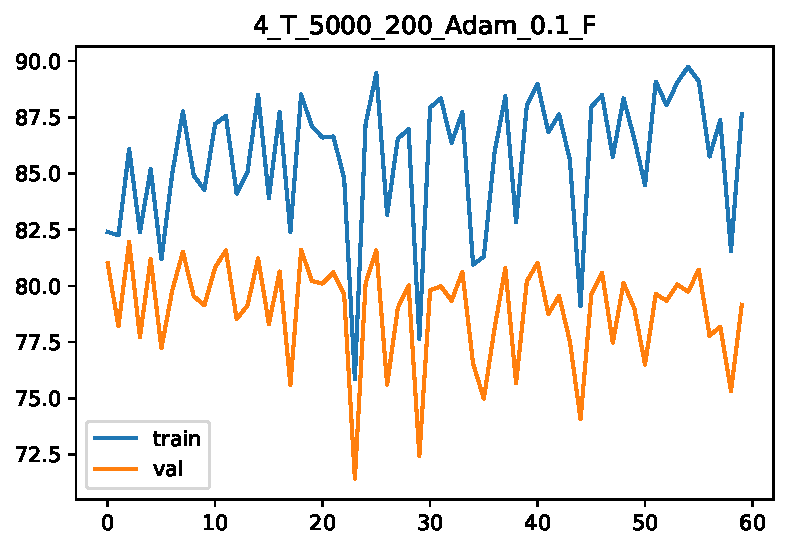
\includegraphics[width = 3cm]{4_T_5000_200_Adam_01_F.pdf}
%}
%\subfloat[(Adam,T,0.1)]{
%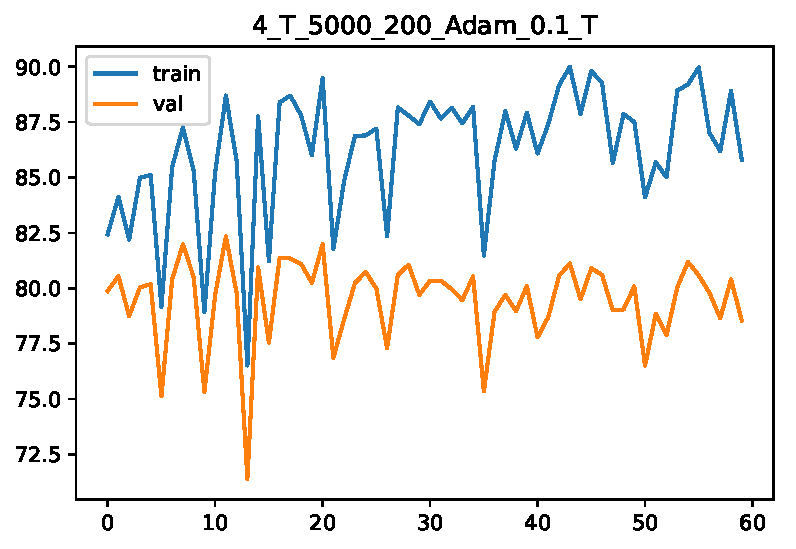
\includegraphics[width = 3cm]{4_T_5000_200_Adam_01_T.pdf}
%}	
%\subfloat[(SGD,F,0.1)]{
%\includegraphics[width = 3cm]{2_F_5000_200_SGD_01_F.pdf}
%}
%\subfloat[(SGD,T,0.1)]{
%\includegraphics[width = 3cm]{2_F_5000_200_SGD_01_T.pdf}
%}
%\caption{\label{fig:optim}Vary Optimization and Fix the Others Learning Curves.}
%\end{figure}
\subsection{Best Hyperparameters and Test Accuracy}
After ablation hyperparameters search, we have the best hyperparameters combination for both CNN and RNN. They are:
\begin{itemize}
\item \textbf{CNN}	\texttt{hidden\_size} = 300, \texttt{is\_concat} = True, \texttt{kernel\_size} = 3, \texttt{is\_wd} = False, \texttt{is\_dropout} = False. \textbf{Validation Accuracy: 65.0}  
\item \textbf{RNN}	\texttt{hidden\_size} = 400, \texttt{is\_concat} = False,  \texttt{is\_wd} = False, \texttt{is\_dropout} = True. \textbf{Validation Accuracy: 73.9}  
\end{itemize}
 
\subsection{List 3 Correct Predictions and 3 Incorrect Predictions}
Correct Predictions. 
\begin{itemize}
\item \textbf{Entailment}. `bicycles stationed while a group of people socialize .'
 `People get together near a stand of bicycles .'
\item \textbf{Contradiction}. `Man in white shirt and blue jeans looking to the side while walking down a busy sidewalk .',
 `Man has a blue shirt on .'
\item \textbf{Neutral}. 'A little boy watches a Ferris Wheel in motion .',
 'A boy is waiting in line for the Ferris Wheel .'
\end{itemize}
Incorrect Predictions. 
\begin{itemize}
\item \textbf{Entailment predicted as Contradiction} `Two people are in a green forest .', `The forest is not dead .' \textbf{Possible Reason}: Since `dead' and `green' are opposite words, it is possible for the network not to learn that the `not dead' and `green' are the same; and we do not use bi-gram.
\item \textbf{Contradiction predicted as Neutral}`Two women , one walking her dog the other pushing a stroller .', `There is a snowstorm .' \textbf{Possible Reason}: This contradiction is not obvious. The network could hardly get that `walking a dog' is not possible in a snowstorm. There is no obvious contradicted word or phrase pair.
\item \textbf{Neutral predicted as Contradiction}`A group of numbered participants walk down the street together .',
 `Participants wait for the beginning of the walkathon .' \textbf{Possible Reason}: `wait' and `walk down the street' looks like a contradicted pair. 
\end{itemize}

\subsection{Evaluating on MultiNLI}
There are five different genres: `fiction', `telephone', `slate', `government', and `travel'. We show the accuracy for different genes. We test our best RNN and CNN model on the MultiNLI validation set. The results are shown in \ref{tab: val}. The accuracies on the new dataset is much lower than the old dataset. And the accuracies from different genres are similar but not the same. Some of the genres have higher accuracy for RNN and some have higher accuracy for CNN. They do not overlap. The conclusion is that the trained model learned may not have very good performance on a dataset with different distribution. 
\begin{table}[!ht]
\centering
\begin{tabular}{|c|c|c|c|c|c|}
\hline
Genre & fiction & telephone & slate & government & travel\\ \hline
Accuracy (RNN) & 41.2 & 42.0 & 38.1 & 39.5 & 39.7 \\ \hline
Accuracy (CNN) & 39.2 & 37.2 & 39.5 & 37.6 & 39.0 \\ \hline
\end{tabular}
\caption{\label{tab: val}Accuracy on MultiNLI Validation Set for best CNN and RNN model.}
\end{table}
\clearpage
\section{Bonus: Fine tune on new data set}
We load the best RNN model and train it for 5 epochs to fine-tune for each genre. We get accuracy in Table \ref{tab: ft}. We also show the accuracy for training without loading the pretrained model (Plain Training). It is very bad. So Fine-Tuning does play an important part in training on small dataset.
\begin{table}[!ht]
\centering
\begin{tabular}{|c|c|c|c|c|c|}
\hline
Genre & fiction & telephone & slate & government & travel\\ \hline
Accuracy (RNN) & 41.2 & 42.0 & 38.1 & 39.5 & 39.7 \\ \hline
Accuracy (RNN) Fine Tune & 45.3 & 50.7 & 43.7 & 53.3 & 49.7 \\ \hline
Accuracy (RNN) Plain Training & 34.5 & 36.1 & 35.9 & 29.9& 36.0 \\ \hline
\end{tabular}
\caption{\label{tab: ft}Accuracy on MultiNLI Validation Set for best CNN and RNN model.}
\end{table}
\end{document}







